\chapter{几何算子、热核与边界响应}
\label{chap:ghs-math-geometric-operators}
\label{chap:ghs-conformal-radial-geometry}
\label{chap:ghs-general-conformal-geometry}

联络、体积测度和超曲面的法向已经确定几何微分的含义；自伴域与谱测度又规定了哪些微分表达式真正成为算子。两类结构汇合以后，才能计算空间中的扩散核、逆算子和边界响应。

热参数以长度平方计，它与 Lorentz 时间及圆锥上的对数径向坐标分别定义。先建立丛值热核及其误差，再研究共形变换和径向酉约化，最后将内区解压缩为边界上的算子。

\section{联络算子与齐性截面的谱}

设 $(M,g)$ 是光滑 $n$ 维黎曼流形，$E\to M$ 是秩为 $r$ 的实或复向量丛，纤维内积记作 $\langle\cdot,\cdot\rangle_E$。一阶联络 $\nabla^E$ 满足 $\nabla^E(fu)=\dd f\otimes u+f\nabla^Eu$；若它与纤维内积相容，则沿曲线的平行移动保持范数。联络的曲率不是数值函数，而是纤维上的线性变换
\begin{equation}\label{eq:ghs-r6-bundle-curvature}
F_{ab}u=([\nabla^E_a,\nabla^E_b]-\nabla^E_{[\partial_a,\partial_b]})u.
\end{equation}
在坐标基中第二项消失。若 $E=T^*M$，$F$ 便是 Riemann 曲率对协变指标的作用；若 $E$ 是带内部表示的丛，它还可以包含规范场强。因此同一个公式适用于标量、张量以及有内部指标的场。

\begin{definition}[联络拉普拉斯算子]
在紧支光滑截面上定义 $\nabla^{E*}$ 为 $\nabla^E$ 在 $L^2$ 内积下的形式伴随。非负的联络拉普拉斯算子为
\begin{equation}\label{eq:ghs-r6-bochner-laplacian}
\nabla^{E*}\nabla^Eu=-g^{ab}(\nabla^E_a\nabla^E_b-\Gamma^c{}_{ab}\nabla^E_c)u.
\end{equation}
对于自伴丛端同态 $V\in\Gamma(\operatorname{End}E)$，算子 $A=\nabla^{E*}\nabla^E+V$ 称为拉普拉斯型算子。
\end{definition}

这个定义从主符号中把几何与动力学分开：最高二阶项是 $|\xi|_g^2\operatorname{id}_E$，而 $V$ 只影响低阶谱修正。采用紧支截面可将分部积分的边界项暂时移走。在无边界紧致流形上，
\[
\langle\nabla^{E*}\nabla^Eu, u\rangle_{L^2}
 =\int_M|\nabla^Eu|_g^2\dd\mu_g\ge0.
\]
若有边界，等式右侧还要连同指定的边界条件一起解释，不能仅凭微分表达式宣称算子正或自伴。


\begin{proposition}[规范齐性联络的 Casimir 差]
设 $G$ 为紧 Lie 群，$H\subset G$ 为闭子群，$\rho:H\to U(V_\rho)$ 为纤维酉表示。对应齐性丛是 $E=G\times_HV_\rho\to G/H$；其截面以等变函数 $f(gk)=\rho(k)^{-1}f(g)$ 表示。对这个纤维表示 $V_\rho$，设 $G$ 上取双不变内积，$\mathfrak g=\mathfrak h\oplus\mathfrak m$ 为正交分解，并用 $\mathfrak m$ 诱导 $G/H$ 上的正规齐性度规。对 $V_\rho$ 取来自 $H$ 的规范齐性联络。选 $\mathfrak g$ 的一组正交基，其 Casimir 二次算子记为 $C_G$；对 $H$ 同样定义 $C_H$。按左正则作用的标准正号，规范联络粗拉普拉斯在每个 $V_\lambda$ 型上的本征值满足
\begin{equation}\label{eq:ghs-r6-casimir-bundle-laplacian}
\lambda_{\lambda,V}=C_G(\lambda)-C_H(V_\rho)
\end{equation}
（若 $V_\rho$ 可约，则须在每个 $H$ 不可约分量上分别解释）。这条公式依赖规范齐性联络与正规齐性度规；对任意变形度规或任意附加规范场并不普遍成立。

\end{proposition}
\begin{proof}
让 $R_X$ 表示右微分，沿 $\mathfrak m$ 的水平导数给出粗拉普拉斯的主项 $-\sum_{i\in\mathfrak m}R_{X_i}^2$。完整群 Casimir 可按正交基拆为
\[
-\sum_{i\in\mathfrak g}R_{X_i}^2
=-\sum_{i\in\mathfrak m}R_{X_i}^2-\sum_{a\in\mathfrak h}R_{Y_a}^2.
\]
对等变函数 $f(gk)=\rho(k)^{-1}f(g)$ 沿 $Y_a\in\mathfrak h$ 求导，得 $R_{Y_a}f=-\rho_*(Y_a)f$。于是纤维方向的正 Casimir 等于 $-\sum_a\rho_*(Y_a)^2=C_H(V_\rho)$。将该项从群 Casimir 中减去，正得到水平拉普拉斯的本征值。规范化若整体改变度规长度，两个 Casimir 必须一同按长度平方重新定标。
\end{proof}

对 $S^2\simeq SO(3)/SO(2)$，平凡的 $SO(2)$ 纤维表示对应通常标量球谐。$SO(3)$ 自旋 $\ell$ 表示的 Casimir 为 $\ell(\ell+1)$，其对 $SO(2)$ 的权 $0$ 子空间恰一维。因此每个 $\ell=0,1,2,\ldots$ 出现一次 $SO(3)$ 表示，贡献 $2\ell+1$ 个磁量子数。单位二球上的本征值与简并度于是同时从 齐性丛截面的表示重数公式 $\dim\operatorname{Hom}_H(V_\ell,V_\rho)$（《群论》的齐性空间章节给出一般证明） 得到。

若纤维改为 $SO(2)$ 的整数权 $s$ 线表示，则只有 $\ell\ge|s|$ 的 $SO(3)$ 表示包含该权，而且该权仍恰出现一次。规范齐性联络下的谱变成
\begin{equation}\label{eq:ghs-r6-spinweighted-laplacian}
\lambda_{\ell,s}=\ell(\ell+1)-s^2,
\qquad \ell=|s|,|s|+1,\ldots,
\end{equation}
每个本征值的表示重数为 $2\ell+1$。它是带权线丛上的粗拉普拉斯，而不是把普通标量拉普拉斯无条件作用于所谓的“带自旋球谐”。若求的是自旋升降算子、Hodge 拉普拉斯算子或 Lichnerowicz 拉普拉斯算子，它们还可能带有明确的曲率位移项。

例如，在一形式上的 Weitzenbock 差异的计算中，
对任何黎曼流形上的一形式 $\alpha$，Hodge 拉普拉斯算子满足
\begin{equation}\label{eq:ghs-r6-weitzenbock-oneform}
(\dd\delta+\delta\dd)\alpha=\nabla^*\nabla\alpha+\operatorname{Ric}(\alpha).
\end{equation}
若 $\alpha=\dd f$ 且 $-\Delta f=\lambda f$，则 Hodge 拉普拉斯算子与 $\dd$ 交换，故 $\Delta_H(\dd f)=\lambda\dd f$；在单位二球上 $\operatorname{Ric}=g$，所以 $\nabla^*\nabla(\dd f)=(\lambda-1)\dd f$。同一个一形式模态对两种自然算子有相差 $1$ 的谱，说明不注明算子类型便引用“高自旋球谐本征值”是不够严格的。

高自旋场最一般的定义涉及张量或自旋表示纤维，而不是一个大本征值。若 $E=\operatorname{Sym}_0^S(T^*X)$，自旋 $S$ 是每一点纤维的对称无迹张量类型。若 $X$ 具有群作用，截面 Hilbert 空间又可以按 $G$ 的全局表示 $\lambda$ 分解。这两个标签性质不同：前者即使没有空间等距群也存在，后者要求明确的对称群作用。只有在额外的表示对应与动力学条件下，才可把某一个大 $\lambda$ 极限解释为球面对称模型中的大角动量极限。

对于非齐性空间，一般无法将各本征值按某个 $SO(d)$ 自旋编号，但对自伴椭圆算子仍有谱投影、极小极大变分原理和热核渐近。若 $A$ 的闭二次型为 $q$，紧致条件下其第 $k$ 个本征值可写成
\begin{equation}\label{eq:ghs-r6-minmax-eigen}
\lambda_k=\inf_{\substack{L\subset\operatorname{Dom}(q)\\\dim L=k}}
\ \sup_{\substack{0\ne u\in L}}\frac{q[u]}{\norm{u}^2}.
\end{equation}
它的普适性来自算子的自伴性和紧预解性，而非高对称群。对度规或势的微小扰动，可用此变分式讨论谱稳定性；若某个本征值高度简并，还必须在简并子空间内对扰动进行矩阵对角化，不能只使用非简并微扰公式。

当 $\Sigma$ 不齐性时，$L^2(\Sigma)$ 不再天然携带上述 $G/H$ 分解。若 $\Sigma$ 只有离散等距群，仍可按有限群表示组织某些简并态；若无对称，通常只能按自伴算子的谱测度组织态。局部 $SO(d-1)$ 标架表示并没有消失，但它不再构成全局守恒角动量。要研究这种局部表示怎样随位置移动，就必须引入联络与曲率。

一般空间上的张量截面表示 $\operatorname{Sym}_0^S$，与平直共形场论中一个标度维数 $\Delta$、自旋 $S$ 的初级算符尚不是同一概念。后者还要求尺度生成元与特殊共形生成元及其交换关系存在，并且初级态被 $K_\mu$ 湮灭。在缺少共形对称的齐性空间中，Casimir 可以帮助对角化某些波动算子，但不会凭空产生 $D$ 或共形后裔塔。前面已建立的几何谱分解提供了严格的起点，之后只有在相应对称条件满足时，才能进入平直背景上的径向共形表示论。

等距群的不可约表示给出了角向谱的简并度，却还没有告诉我们一块局部张量场的哪些分量是物理自由度。自旋首先是正交标架群的表示；只有确定它所在的向量丛以及协变导数，才能把高自旋的动力学写在一般背景上。
\begin{figure}[htbp]
\centering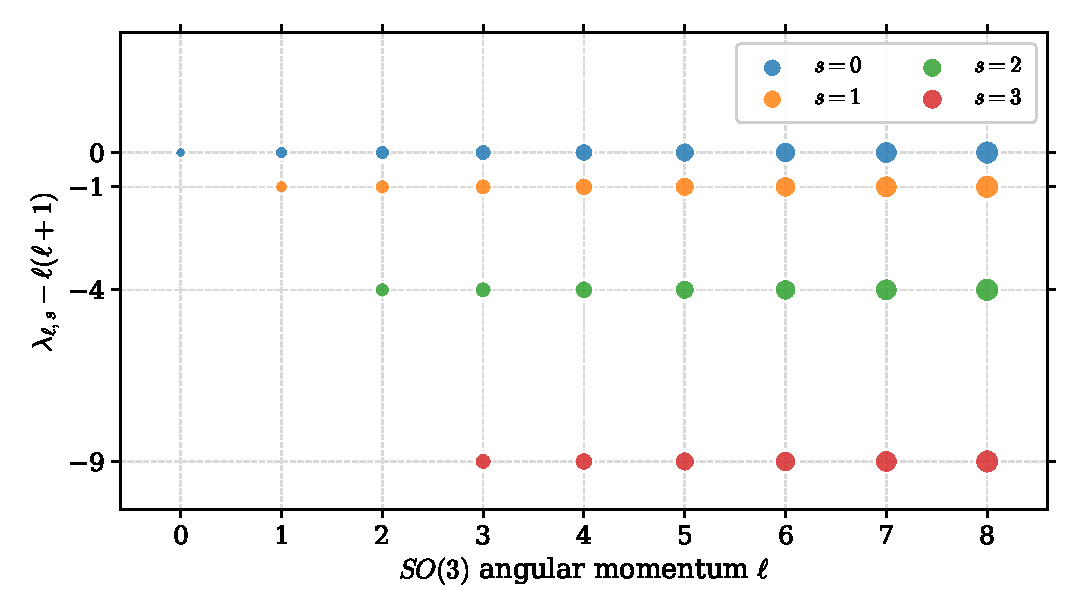
\includegraphics[width=.83\linewidth]{content/MathSkills/figures/geometry-highspin/spin_weight_bundle_spectrum.pdf}
\caption{单位二球带整数权 $s$ 的齐性线丛粗拉普拉斯谱 $\lambda_{\ell,s}=\ell(\ell+1)-s^2$。纵坐标是相对于标量 Casimir 的位移 $\lambda_{\ell,s}-\ell(\ell+1)=-s^2$，点大小与简并度 $2\ell+1$ 成正比，左端缺失的点体现最低允许 $\ell=|s|$。此图不是 Hodge 拉普拉斯算子的全部一形式谱，更不能将 $s$ 当作平直环面上的 Fourier 波矢。}\label{fig:ghs-r9-spin-weight-spectrum}
\end{figure}

\cref{fig:ghs-r9-spin-weight-spectrum} 把前文的齐性空间重数公式变成可阅读的谱图：同样是“自旋”，球面的局部纤维权 $s$ 通过稳定子表示限制允许出现的 $SO(3)$ 角动量 $\ell$；环面上的纵横分解却来自外微分代数。二者可以在同一高自旋问题中同时出现，但数学上不是同一个分解。

\section{热半群、热迹与局域几何}
在同一纤维内作酉基底变换，只会改变算子的矩阵表示，并不会改变它的谱。

\begin{proposition}[酉丛变换与谱不变性]
\label{prop:ghs-r6-gauge-unitary}
设 $U:E\to E$ 是光滑的逐点酉丛自同构，并令 $\nabla'=U\nabla^EU^{-1}$、$V'=UVU^{-1}$。在映到彼此的算子定义域上，$A'=UAU^{-1}$；因而二者的谱测度、重数及热迹（若存在）相同。

\end{proposition}
\begin{proof}
对任意截面 $u$，$\nabla'(Uu)=U\nabla^Eu$。由于 $U$ 保持纤维内积和体积测度，取形式伴随后有 $\nabla'{}^*(U\alpha)=U\nabla^{E*}\alpha$，再作用一次即得 $A'(Uu)=UAu$。若边界条件也由 $U$ 传送，$U$ 将闭算子的定义域双射到新定义域，故 $A'$ 与 $A$ 酉等价。对 Borel 函数 $f$，谱演算还给出 $f(A')=Uf(A)U^{-1}$，结论成立。
\end{proof}

设 $A$ 是下有界自伴实现，先减去一个常数使 $A\ge0$。谱定理给出投影值测度 $\mathsf E_A$，以及
\begin{equation}\label{eq:ghs-r6-heat-functional-calculus}
T(t)=\ee^{-tA}=\int_{[0,\infty)}\ee^{-t\lambda}\,\dd\mathsf E_A(\lambda),\qquad t\ge0.
\end{equation}
这里 $t$ 的量纲是长度平方；它是热演化参数，不是物理时间。由谱积分相乘可知 $T(t+s)=T(t)T(s)$、$\norm{T(t)}\le1$，并且 $T(t)$ 在 $t\downarrow0$ 时强收敛到恒等算子。若 $A$ 的谱离散且本征截面 $u_j$ 构成完备正交基，
\[
T(t)f=\sum_j\ee^{-t\lambda_j}\langle f, u_j\rangle u_j,
\qquad H_t(x,y)=\sum_j\ee^{-t\lambda_j}u_j(x)u_j(y)^*.
\]
第二式中的 $H_t(x,y)$ 是从 $E_y$ 到 $E_x$ 的线性映射；不能把向量丛值热核误写成没有平行移动意义的标量函数。

\begin{figure}[htbp]
\centering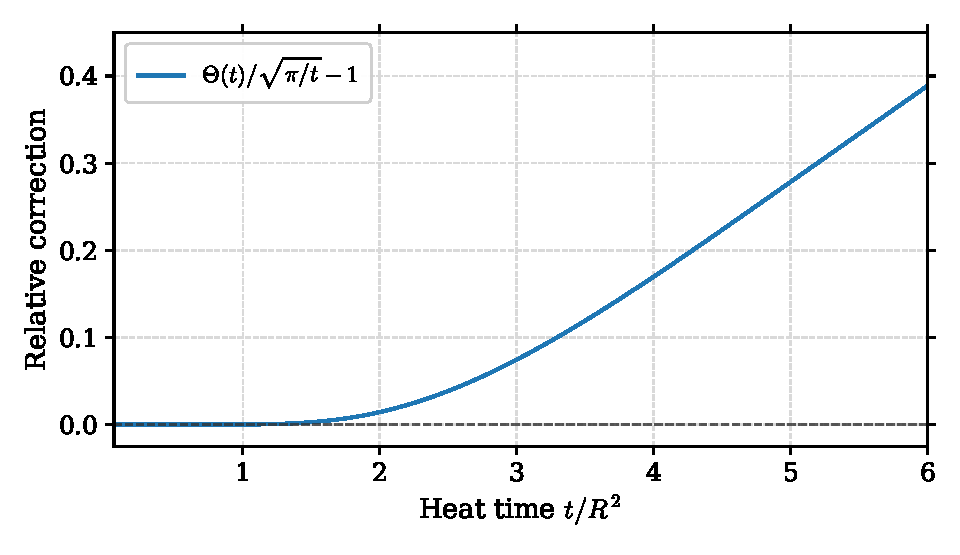
\includegraphics[width=.79\linewidth]{content/MathSkills/figures/geometry-highspin/heat_trace_circle.pdf}
\caption{单位半径圆周上的精确热迹 $\Theta(t)=\sum_{n\in\ZZ}\ee^{-n^2t}$ 与 Weyl 主项 $\sqrt{\pi/t}$ 的相对偏差。零参考线表示局部 Weyl 预测；短热时间的领先偏差由 Poisson 求和中的 $2\ee^{-\pi^2/t}$ 控制。}\label{fig:ghs-heat-trace-circle}
\end{figure}

\cref{fig:ghs-heat-trace-circle} 使热核与全局拓扑之间的关系可见：$t\downarrow0$ 时先读到局部体积，闭合路径的影响则以 $\ee^{-\pi^2/t}$ 的非幂级数方式出现。

\begin{theorem}[热核拼接与正算子性质]\label{thm:ghs-r6-heat-gluing}
若 $A$ 在紧致无边界流形上是非负自伴拉普拉斯型算子，则 $t>0$ 时热核光滑，并满足
\begin{equation}\label{eq:ghs-r6-heat-convolution}
H_{t+s}(x,y)=\int_MH_t(x,z)H_s(z,y)\dd\mu_g(z),
\qquad H_t(x,y)^*=H_t(y,x).
\end{equation}
当纤维秩为 $1$ 且 $A=-\Delta+V$、$V$ 为实函数时，正性保持的半群还满足正数据不会产生负值的性质；对任意向量丛上的矩阵势不能仅从 $A\ge0$ 推出逐分量非负。
\end{theorem}
\begin{proof}
谱演算给 $T(t+s)=T(t)T(s)$。将两个积分核逐次作用于测试截面并运用 Fubini 定理，就得到第一式；对有限谱截断可逐项验证，再使用光滑性和适当核收敛完成极限。自伴性给 $T(t)^*=T(t)$，故得到第二式。标量正性保持可由热方程的最大值原理证明；丛值截面没有自然的逐点全序，最后的区别来自这一基本事实。
\end{proof}

高能谱为什么只在领先阶感受到体积，而较低阶逐渐感受到曲率？在短热时间中，热量只能沿很短的测地线传播，因此热核接近欧氏空间上的 高斯 核。取正算子 $A=\nabla^{E*}\nabla^E+V$，在紧致无边界光滑流形上有渐近式
\begin{equation}\label{eq:ghs-r6-heat-local-coefficients}
\operatorname{Tr}_{E_x}H_t(x,x)\sim\frac1{(4\pi t)^{n/2}}
\operatorname{tr}_E\left[\id+t\left(\frac{\mathcal R}{6}\id-V\right)+O(t^2)\right].
\end{equation}
此处 $\mathcal R$ 是标量曲率。$O(t^2)$ 应按局部光滑渐近展开理解，不保证该级数对固定 $t$ 收敛。若使用 $A=-(g^{ab}\nabla_a\nabla_b+\mathcal E)$ 的常见另一种约定，$V=-\mathcal E$，所以一次系数应写 $\mathcal E+\mathcal R/6$；符号不能在两个约定之间随意搬用。

我们先解释可直接计算的 $V$ 项。设平直空间上 $V=v$ 是常数，则 Fourier 变换把 $A=-\Delta+v$ 化为乘法 $|k|^2+v$，从而
\[
H_t(x,x)=\int_{\RR^n}\frac{\dd^nk}{(2\pi)^n}\ee^{-t(|k|^2+v)}
=(4\pi t)^{-n/2}\ee^{-tv}
=(4\pi t)^{-n/2}(1-tv+O(t^2)).
\]
这一步固定了势项的负号。曲率项 $\mathcal R/6$ 则来自法坐标中 高斯 传播与体积 雅可比因子 的二阶修正；一般情形需要将测地世界函数、Van Vleck 行列式和热方程递推一起处理，不能仅对体积因子做 Taylor 展开便声称证明了完整系数。相应的标准局部热核构造可参照 \cite{r6-vassilevich,r6-gilkey} 中的参数核方法。

在两个点由唯一短测地线连接的凸正规邻域内，定义半测地距离平方
$\Sigma(x,y)=\tfrac12\operatorname{dist}_g(x,y)^2$，令 $D_a$ 表示 $E$ 上的联络。它满足 eikonal 恒等式
\[
 g^{ab}(D_a\Sigma)(D_b\Sigma)=2\Sigma.
\]
为使局部核的最高短时间行为与欧氏 高斯 相同，设
\begin{equation}\label{eq:ghs-r6-parametrix-ansatz}
H_t(x,y)\sim (4\pi t)^{-n/2}\ee^{-\Sigma(x,y)/(2t)}
\sum_{j\ge0}t^ja_j(x,y),
\end{equation}
其中 $a_j(x,y):E_y\to E_x$，对一般向量丛不能把它们当作无指标的数。先求指数的一阶、二阶协变导数：
\begin{align*}
D_a\ee^{-\Sigma/(2t)}
&=-\frac{D_a\Sigma}{2t}\ee^{-\Sigma/(2t)},\\
D^aD_a\ee^{-\Sigma/(2t)}
&=\left[\frac{|D\Sigma|^2}{4t^2}
 -\frac{\Delta\Sigma}{2t}\right]\ee^{-\Sigma/(2t)}.
\end{align*}
对任意丛值振幅 $a$ 使用乘积法则，则
\[
D^aD_a(\ee^{-\Sigma/(2t)}a)
=\ee^{-\Sigma/(2t)}\left[D^aD_aa
 -\frac{D^a\Sigma}{t}D_aa
 +\left(\frac{2\Sigma}{4t^2}-\frac{\Delta\Sigma}{2t}\right)a\right].
\]
把 \cref{eq:ghs-r6-parametrix-ansatz} 代入热方程 $(\partial_t+A_x)H_t=0$，其中 $A=-D^aD_a+V$。$t^{-2}$ 项来自指数的时间导数和空间 拉普拉斯算子；由于 eikonal 恒等式，它们恰好抵消。$t^{-1}$ 阶得到领先运输方程
\begin{equation}\label{eq:ghs-r6-heat-a0-transport}
\left[2D^a\Sigma D_a+\Delta\Sigma-n\right]a_0=0,
\qquad a_0(y,y)=\id.
\end{equation}
匹配其后 $t^{j-1}$ 系数，得到递推式
\begin{equation}\label{eq:ghs-r6-heat-aj-transport}
\left[2D^a\Sigma D_a+\Delta\Sigma-n+2j\right]a_j
=2(D^aD_a-V)a_{j-1},\qquad j\ge1.
\end{equation}
这一关系是局部渐近构造的真正动力：每一级系数都由前一级沿测地线的输运决定，而不是逐阶猜测曲率不变量。

当 $x\to y$ 时有 $D\Sigma=0$、$\Delta\Sigma=n$，所以对于 $j=1$，
$a_1(y,y)=(D^aD_aa_0)(y,y)-V(y)$。在 $y$ 的测地法坐标与平行纤维框架中，\cref{eq:ghs-r6-heat-a0-transport} 的解为
\[
a_0(x,y)=\Delta_{\rm VM}(x,y)^{1/2}\mathcal P_{y\to x},
\]
其中 $\mathcal P_{y\to x}$ 是联络平行移动，$\Delta_{\rm VM}$ 是 Van Vleck 行列式。

用 Jacobi 场与正规坐标的体积膨胀可得到
\[
\Delta_{\rm VM}(x,y)^{1/2}
=1+\frac1{12}\operatorname{Ric}_{ab}(y)x^ax^b+O(|x|^3).
\]
平行框架中平行移动对角点的 拉普拉斯算子 收缩没有附加一阶曲率项，因为联络曲率在导数指标上反对称。于是
\[
(D^aD_aa_0)(y,y)=\frac16\mathcal R(y)\id,
\quad a_1(y,y)=\frac16\mathcal R(y)\id-V(y),
\]
恰好恢复 \cref{eq:ghs-r6-heat-local-coefficients}。

这证明了局部一次热核系数；关于余项在一般几何上的一致控制仍需参数核误差估计。

\begin{proposition}[热迹控制 Weyl 系数]\label{prop:ghs-r6-tauberian-weyl}
若 $A$ 在秩 $r$ 的丛上为非负椭圆拉普拉斯型算子，$M$ 紧致无边界，则
\begin{equation}\label{eq:ghs-r6-leading-weyl}
N_A(\Lambda)\sim\frac{r\,\omega_n\operatorname{Vol}(M)}{(2\pi)^n}\Lambda^{n/2}
\qquad(\Lambda\to\infty).
\end{equation}
\end{proposition}
\begin{proof}
对谱计数测度 $\dd N_A$，热迹恰为其 Laplace 变换：
\[
\operatorname{Tr}(\ee^{-tA})=\sum_j\ee^{-t\lambda_j}
=\int_{[0,\infty)}\ee^{-t\lambda}\,\dd N_A(\lambda).
\]
将 \cref{eq:ghs-r6-heat-local-coefficients} 的主项沿 $M$ 积分得
$\operatorname{Tr}(\ee^{-tA})\sim r\operatorname{Vol}(M)(4\pi t)^{-n/2}$。
非减函数的 Tauber 定理把这一热迹渐近变为
$N_A(\Lambda)\sim r\operatorname{Vol}(M)\Lambda^{n/2}/[(4\pi)^{n/2}\Gamma(1+n/2)]$。
由于 $\omega_n=\pi^{n/2}/\Gamma(1+n/2)$，即为所列公式。最后一步调用 Tauber 定理而非简单逐项逆 Laplace 变换；原因是点态谱计数含阶梯函数。
\end{proof}

\subsection{二球热核与角动量截断}
\label{sec:ghs-heat-kernel-boundary}

若 $A\ge m^2>0$，对每个谱值都有 $\lambda^{-1}=\int_0^\infty\ee^{-t\lambda}\dd t$，从而
\begin{equation}\label{eq:ghs-r6-green-propertime}
A^{-1}=\int_0^\infty\ee^{-tA}\dd t.
\end{equation}
这里积分在算子范数中收敛，其范数由 $m^{-2}$ 控制。若 $A\ge0$ 但有非平凡零模，原积分沿零模发散；在紧致情形应先定义正交投影 $\Pi_0$，改用
\[
A^+=\int_0^\infty\bigl(\ee^{-tA}-\Pi_0\bigr)\dd t.
\]
该式还需正谱离零有间隙；对连续谱逼近零点的非紧空间，一般只能在指定的加权空间、二次型或分布意义下解释。这是算子定义域与红外行为不能分开的一个例子。

例如，在圆周与球面的热迹的计算中，
\label{ex:ghs-r6-circle-heat}
长度为 $L$ 的平直圆周有 $\lambda_k=(2\pi k/L)^2$。Poisson 求和给出
\[
\sum_{k\in\ZZ}\ee^{-4\pi^2tk^2/L^2}
=\frac{L}{\sqrt{4\pi t}}\sum_{m\in\ZZ}\ee^{-m^2L^2/(4t)}.
\]
因此 $t\downarrow0$ 时主项是 $L/\sqrt{4\pi t}$，其余修正指数小；一维圆周的局部曲率为零。标准单位二球则有 $\lambda_\ell=\ell(\ell+1)$、重数 $2\ell+1$，热迹领先项 $\operatorname{Area}(S^2)/(4\pi t)=t^{-1}$，并有来自 $\mathcal R/6=1/3$ 的常数项。两个例子说明曲率、拓扑与空间维数以不同阶次进入谱。

\begin{figure}[htbp]
\centering
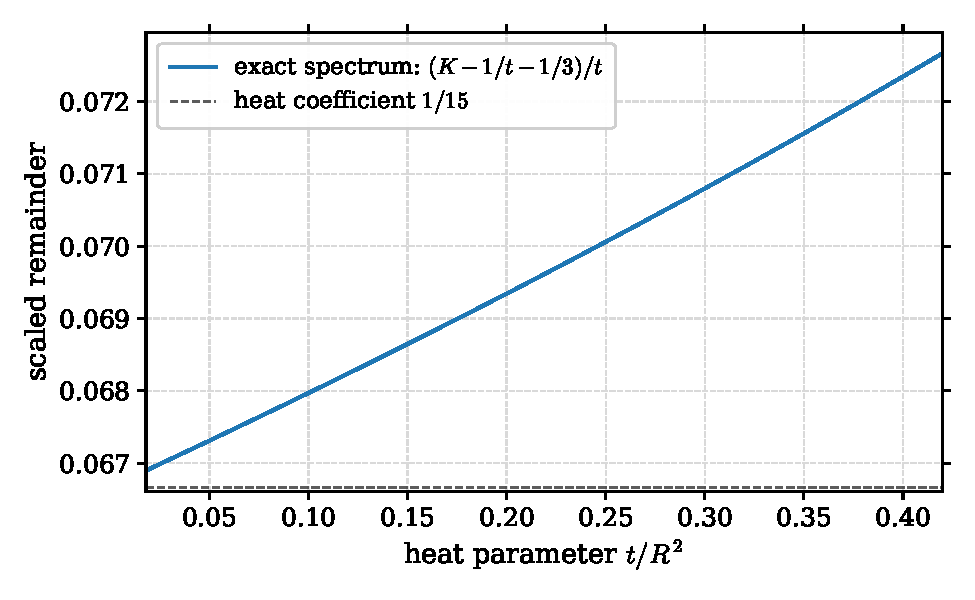
\includegraphics[width=.78\linewidth]{content/MathSkills/figures/geometry-highspin/heat_curvature_remainder.pdf}
\caption{单位二球热迹去掉 Weyl 主项 $t^{-1}$ 和曲率常数项 $1/3$ 后的缩放余项。精确谱求和趋向下一阶系数 $1/15$，显示不同几何数据进入不同的热时间阶数。}
\label{fig:ghs-r6-heat-remainder}
\end{figure}

一般向量丛热核的参数核需要联络与曲率输运，初次接触时很容易变成一串抽象系数。单位二球是一个有用的完整算例：它不仅有离散谱，而且存在可以直接把全部模态求和为一个按测地距离变化的核的加法定理。借此既能看见扩散的空间形状，也能检验短时间曲率系数与截断误差。

令 $\Sigma=S_R^2$ 为半径 $R$ 的标准球面，令 $A=-\Delta_{S_R^2}$ 作用于标量，热参数 $t>0$ 的单位为长度平方。球谐满足
\[
 AY_{\ell m}=\frac{\ell(\ell+1)}{R^2}Y_{\ell m},\qquad
 \sum_{m=-\ell}^{\ell}|Y_{\ell m}(x)|^2=\frac{2\ell+1}{4\pi R^2}.
\]
这里球谐按 $\int_{S_R^2}|Y_{\ell m}|^2\dd\mu=1$ 归一化，因而与单位球面常用的球谐相差一个 $R^{-1}$。

对两个点 $x,y$，定义 $\theta=d(x,y)/R\in[0,\pi]$。旋转不变性说明 $\sum_mY_{\ell m}(x)\overline{Y_{\ell m}(y)}$ 只能依赖 $\theta$；在北极 $x$ 固定后解 Legendre 方程，并取 $\theta=0$ 归一，即得到加法定理
\[
 \sum_{m=-\ell}^{\ell}Y_{\ell m}(x)\overline{Y_{\ell m}(y)}
 =\frac{2\ell+1}{4\pi R^2}P_\ell(\cos\theta).
\]

\begin{theorem}[二球热核的精确谱展开]
\label{thm:ghs-r9-sphere-heat}
在无边界的标准二球上，热核 $K_t(x,y)$ 是下列绝对且对 $t\ge t_0>0$ 一致收敛的级数：
\begin{equation}\label{eq:ghs-r9-sphere-heat}
 K_t(\theta)=\frac1{4\pi R^2}\sum_{\ell=0}^{\infty}
 (2\ell+1)\ee^{-t\ell(\ell+1)/R^2}P_\ell(\cos\theta).
\end{equation}
它满足 $\partial_tK_t=\Delta_xK_t$、$K_t(x,y)=K_t(y,x)$、$K_t>0$（$t>0$）及
\begin{equation}\label{eq:ghs-r9-sphere-heat-mass}
 \int_{S_R^2}K_t(x,y)\dd\mu_y=1,
 \qquad \lim_{t\to\infty}K_t(x,y)=\frac1{4\pi R^2}.
\end{equation}
\end{theorem}
\begin{proof}
将 $A$ 的谱定理与加法定理代入 $\ee^{-tA}$ 的积分核便得到 \cref{eq:ghs-r9-sphere-heat}。因为 $|P_\ell(z)|\le1$ 对 $z\in[-1,1]$ 成立，而 $(2\ell+1)\ee^{-t_0\ell(\ell+1)/R^2}$ 可求和，故对 $t\ge t_0$ 一致收敛；逐项微分所需的多项式因子也被指数衰减压住。$\partial_tK_t=\Delta_xK_t$ 由每个本征模态的热方程得出。

质量守恒可直接沿 $y$ 积分：对 $\ell\ge1$，Legendre 正交性给 $\int_{-1}^1P_\ell(z)\dd z=0$，唯有 $\ell=0$ 的积分留下 $1$。长时间极限同样只剩 $\ell=0$。严格的 $K_t>0$ 由连通紧致流形上热方程的强最大值原理得到，而不应仅凭交替符号的 Legendre 级数逐项猜测。
\end{proof}

\begin{figure}[htbp]
\centering% Great-circle cross-section of an S2; geodesic arc vs embedding chord.
\begin{tikzfig}[scale=1.0]
\coordinate (O) at (0,0);
\coordinate (P) at (0,2.15);
\coordinate (Q) at (1.97,.86);
\draw[thick] (O) circle (2.15);
\fill (O) circle (1.7pt);
\fill (P) circle (2.6pt);
\fill (Q) circle (2.6pt);
\draw[gray,dashed] (O)--(P) (O)--(Q);
\draw[gray!70,dashed] (P)--(Q);
\draw[line width=1.6pt] (P) arc[start angle=90,end angle=23.6,radius=2.15];
\draw[lecturearrow] (.0,.74) arc[start angle=90,end angle=23.6,radius=.74];
\node[lecturelabel] at (.50,.94) {$\theta$};
\node[lecturelabel] at (.33,2.54) {Source $x$};
\node[lecturelabel] at (2.58,.85) {Target $y$};
\node[lecturelabel] at (2.9,2.07) {$s=R\theta$};
\node[lecturelabel] at (3.45,-.17) {Chord $2R\sin(\theta/2)$};
\draw[lecturearrow] (1.91,-.05)--(1.20,.70);
\node[lecturelabel] at (-.34,-.34) {$O$};
\node[lecturelabel] at (-1.60,-1.67) {$S_R^2$ section};
\end{tikzfig}

\caption{从球面一点发出的热传播按测地角 $\theta=d(x,y)/R$ 组织，而不是按欧氏弦长 $|x-y|$。球面的闭合性使扩散最终收敛到均匀密度 $1/(4\pi R^2)$；短时间则主要由局部的短测地线控制。}\label{fig:ghs-r9-sphere-heat-geodesic}
\end{figure}
\begin{figure}[htbp]
\centering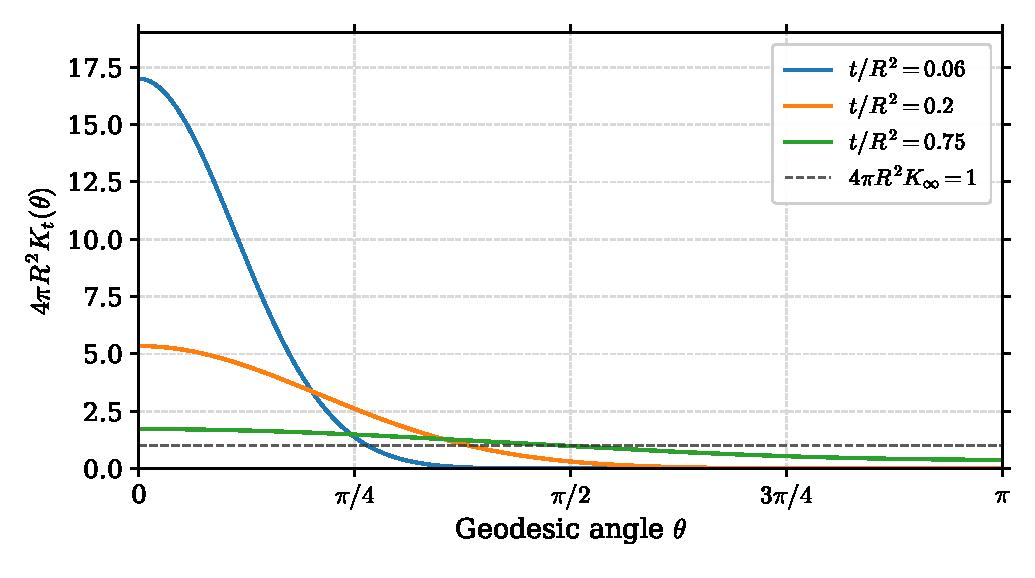
\includegraphics[width=.83\linewidth]{content/MathSkills/figures/geometry-highspin/sphere_heat_geodesic_profiles.pdf}
\caption{半径 $R=1$ 的二球热核，纵轴为 $4\pi R^2K_t(\theta)$，横轴为测地角 $\theta$。曲线由 \cref{eq:ghs-r9-sphere-heat} 的 Legendre 级数直接计算；虚线 $1$ 是保留总概率的长时间均匀极限。越短的热时间越接近局部 高斯，越长的热时间越显现紧致性。}\label{fig:ghs-r9-sphere-heat-profiles}
\end{figure}

短时间的对角热核可以从本章的一般曲率系数独立检查。二球标量曲率为 $\mathcal R=2/R^2$，故
\begin{equation}\label{eq:ghs-r9-sphere-heat-diagonal}
 K_t(0)=\frac1{4\pi t}\left[1+\frac{t}{3R^2}+O\!\left(\frac{t^2}{R^4}\right)\right],
 \qquad t\downarrow0.
\end{equation}
为了不把 $t^{-1}$ 的发散遮住真正的曲率信号，定义无量纲诊断量
\[
 C(q)=\frac{4\pi tK_t(0)-1}{q},\qquad q=t/R^2.
\]
由 \cref{eq:ghs-r9-sphere-heat-diagonal}，$C(q)\to1/3$。继续使用 Euler--Maclaurin 公式对 $F(x)=(2x+1)\ee^{-qx(x+1)}$ 求和，积分项严格为 $\int_0^\infty F(x)\dd x=1/q$，端点修正给出
\begin{equation}\label{eq:ghs-r9-sphere-heat-asymptotic}
 \sum_{\ell\ge0}(2\ell+1)\ee^{-q\ell(\ell+1)}
 =\frac1q+\frac13+\frac q{15}+O(q^2),
 \qquad q\downarrow0.
\end{equation}
于是更精细的残差 $(C(q)-1/3)/q\to1/15$。这一诊断量在有限数值精度下比原始热核更灵敏地暴露曲率项和截断错误。

\begin{figure}[htbp]
\centering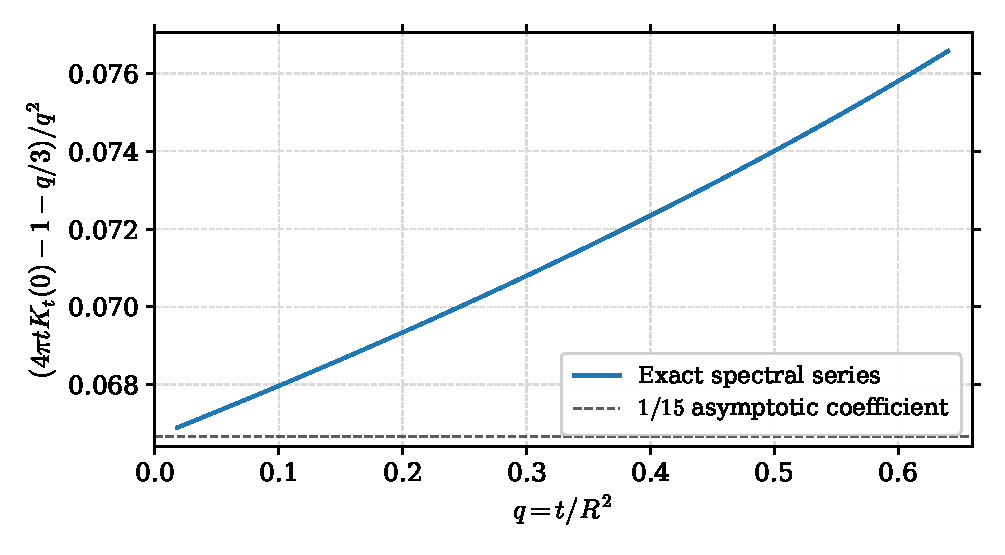
\includegraphics[width=.79\linewidth]{content/MathSkills/figures/geometry-highspin/sphere_heat_curvature_residual.pdf}
\caption{二球对角热核的谱级数数值验证：$[4\pi tK_t(0)-1-q/3]/q^2$ 在 $q=t/R^2\to0$ 时趋于 $1/15$。图采用足够的角动量截断，避免把有限截断的缺失高频模态误读成热核的几何系数。}\label{fig:ghs-r9-sphere-heat-residual}
\end{figure}

\begin{proposition}[热核角动量截断的显式误差]
\label{prop:ghs-r9-sphere-heat-tail}
令 $K_t^{(L_0)}$ 为 \cref{eq:ghs-r9-sphere-heat} 截到 $\ell=L_0$ 的部分和，令 $q=t/R^2$。若 $L_0+1\ge (\sqrt{2/q}-1)/2$，则任意 $\theta\in[0,\pi]$ 都有
\begin{equation}\label{eq:ghs-r9-sphere-heat-tail-bound}
 |K_t(\theta)-K_t^{(L_0)}(\theta)|
 \le \frac{\ee^{-q(L_0+1)(L_0+2)}}{4\pi R^2}
 \left(2L_0+3+\frac1q\right).
\end{equation}
\end{proposition}
\begin{proof}
由 $|P_\ell|\le1$，误差至多为 $\sum_{\ell=L_0+1}^\infty f(\ell)/(4\pi R^2)$，其中 $f(x)=(2x+1)\ee^{-qx(x+1)}$。条件保证 $f'(x)\le0$ 对 $x\ge L_0+1$ 成立，于是积分比较给出
\[
 \sum_{\ell=L_0+1}^{\infty}f(\ell)
 \le f(L_0+1)+\int_{L_0+1}^{\infty}f(x)\dd x.
\]
因为 $\frac{\dd}{\dd x}\ee^{-qx(x+1)}=-qf(x)$，积分恰等于 $q^{-1}\ee^{-q(L_0+1)(L_0+2)}$，代回即得。
\end{proof}

这个误差界给绘图提供了可检查的截断条件，并解释为什么热时间越短，必须保留的高角动量就越多。它仅保证经典球面标量热核的这一谱截断；在一般流形或张量丛上，应以本征值增长及谱投影估计重新建立相应尾界，不能直接沿用 Legendre 多项式的界。

\section{高频计数与半经典传播}
\begin{equation}\label{eq:ghs-weyl-law-sigma}
 N_A(\Lambda)=\frac{\operatorname{Vol}(\Sigma)\,\omega_{d-1}}{(2\pi)^{d-1}}
 \Lambda^{(d-1)/2}+o\bigl(\Lambda^{(d-1)/2}\bigr).
\end{equation}
这里真正普遍的是高能态密度对体积与维数的依赖，而不是球谐的 $\ell(\ell+d-2)$ 本征值。球对称是谱可显式求和的特殊幸运情形。

\begin{figure}[htbp]
\centering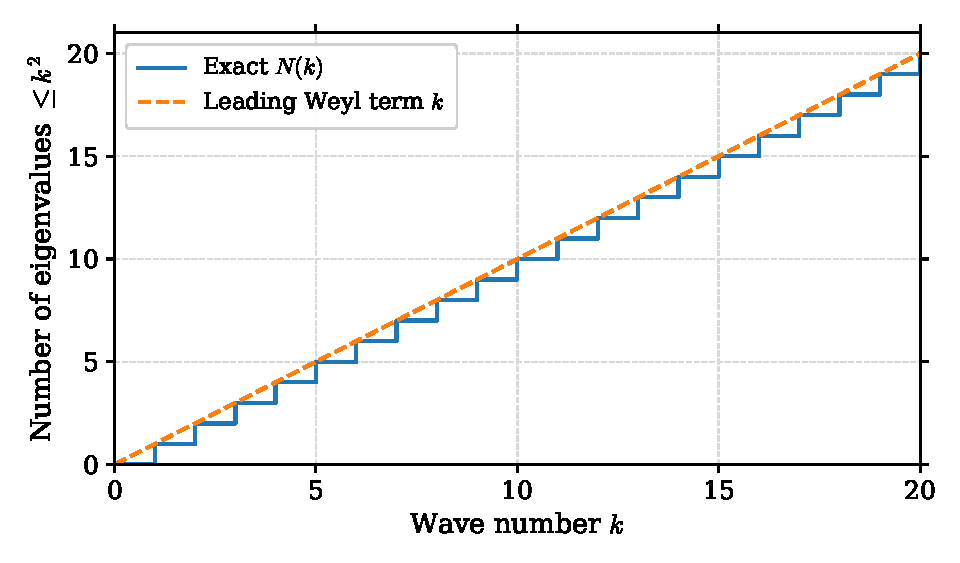
\includegraphics[width=.79\linewidth]{content/MathSkills/figures/geometry-highspin/weyl_staircase.pdf}
\caption{区间 $(0,\pi)$ 上 Dirichlet 算子 $-\partial_x^2$ 的精确阶梯谱计数 $N(k^2)=\lfloor k\rfloor$ 与 Weyl 主项 $k$。竖直跳跃来自离散本征值；主项不解析这些振荡。}\label{fig:ghs-weyl-staircase}
\end{figure}

\cref{fig:ghs-weyl-staircase} 是 Weyl 律的最简单可直接核算的模型，也提醒我们渐近公式给出的是大尺度增长，不会逐个预测本征值。

对高频态的计数，也可以直接按经典相空间体积计算。
在小坐标块中冻结系数，把特征函数近似看成局域平面波。每个相空间量子态占据 $(2\pi)^{d-1}$ 的无量纲相空间体积。满足主符号 $h^{ab}p_ap_b\leq\Lambda$ 的协变量在每点形成椭球；其体积是 $\omega_{d-1}\Lambda^{(d-1)/2}\sqrt{\det h}$。对 $\Sigma$ 积分并除以 $(2\pi)^{d-1}$，得到 \cref{eq:ghs-weyl-law-sigma} 的主项。严格证明还需微局部分析控制坐标块边界与高频误差；这里的相空间计算只用于解释严格 Weyl 定理的系数，不取代其误差证明。

自伴性确定谱演算的数学合法性，而空间对称性决定谱的简并规律。两者不同：即使曲率破坏全部连续等距对称，谱定理仍成立；只是再没有普遍意义上的角动量量子数可用。

高自旋与高频不是同一个概念：前者是群表示标签，后者来自微分算子的谱。如果空间不是球面，未必存在自旋 $S$ 的全局角模态，但仍可以考察 $-\Delta$ 的高本征值极限。半经典分析提供一套几乎不依赖特殊坐标的近似，它将高频传播的主导轨迹联系到测地流，并明确误差何时失去控制。

设 $A_h=-h^2\Delta_g+V$，这里 $h>0$ 是无量纲小参数，与截面度规 $h_{ab}$ 的符号无关。它的经典主符号为
\begin{equation}\label{eq:ghs-semiclassical-principal-symbol}
 p(x,\xi)=g^{ab}(x)\xi_a\xi_b+V(x).
\end{equation}
在余切丛 $T^*M$ 上取典范辛形式 $\dd\xi_a\wedge\dd x^a$，Hamilton 方程为
\[
 \dot x^a=\frac{\partial p}{\partial\xi_a}=2g^{ab}\xi_b,
 \qquad\dot\xi_a=-\frac{\partial p}{\partial x^a}.
\]
当 $V$ 为常数时，轨迹投影到 $M$ 上是重新参数化的测地线。这一结论只用到了局部度规与主符号；不需要旋转群。

考虑定态方程 $A_h\psi=E\psi$，尝试振幅—相位形式 $\psi=a(x)\ee^{\ii S(x)/h}$。对其梯度与 拉普拉斯算子逐步求导，得到
\[
 \nabla_a\psi=\ee^{\ii S/h}
 \left(\nabla_aa+\frac{\ii}{h}a\nabla_aS\right),
\]
\[
 \Delta_g\psi=\ee^{\ii S/h}
 \left[\Delta_ga+\frac{2\ii}{h}\nabla^aS\nabla_aa
 +\frac{\ii}{h}a\Delta_gS-\frac1{h^2}a|\nabla S|_g^2\right].
\]
故原微分方程精确转写为
\begin{equation}\label{eq:ghs-wkb-exact-expansion}
 0=(|\nabla S|_g^2+V-E)a
 -\ii h\left(2\nabla S\cdot\nabla a+a\Delta_gS\right)
 -h^2\Delta_ga.
\end{equation}

第一项给 Hamilton--Jacobi 方程 $|\nabla S|_g^2+V=E$。第二项给振幅输运方程
\[
 2\nabla S\cdot\nabla a+a\Delta_gS=0,
 \qquad\nabla_a\bigl(a^2\nabla^aS\bigr)=0
\]
（当振幅取实时）。第三项 $-h^2\Delta_ga$ 是被舍弃的明确余项；只有当它相对于保留项受控时，近似才有意义。焦散点附近振幅可能发散、相位不再单值，需要新的局部一致近似，而不能继续用同一张 WKB 图遮盖问题。

在紧致无边界截面上，高本征值计数可视为经典能量子集
$\{(x,\xi)\in T^*\Sigma:g^{ab}\xi_a\xi_b\leq\Lambda\}$ 的相空间体积除以 $(2\pi)^{d-1}$，给出 \cref{eq:ghs-weyl-law-sigma} 的领先项。若用 $h\to0$ 参数化，则状态数按 $h^{-(d-1)}$ 增长；这是几何频率的渐近密度，而不是说所有高频本征态在空间上均匀分布。

在标准球面上，最高权谐波因旋转群表示而沿某些大圆附近集中；在其他流形上，局部高频 WKB 可以沿测地轨迹形成集中，但同时可能存在模态疤痕、退化、隧穿或量子遍历性等不同现象。高频谱的总体 Weyl 律并不能单独决定单个本征函数的分布。

因此球面对称自由场模型中“高 $S$ 产生对径峰”的精确公式应始终与其自由、球面对称、特定初级态及场振幅测量的假设绑定。一般空间的正确替代语言是：先指定算子与谱投影，再考察高频、半经典测地流和所选态核的局部集中；未出现角动量表示时，不能强加 $S\to\infty$ 的球面式几何结论。

\section{共形变换与翘曲积的径向约化}




有了任意流形上的微分算子，才可以精确回答“径向量子化为什么偶尔变得特别简单”：当空间的尺度变化可以变成柱面时间平移，而且场方程在 Weyl 变换下具有受控的协变性时，一般随时间变化的背景才简化为静态谱问题。这个性质依赖度规的具体几何，不能单靠把一个坐标命名为 $r$ 得到。

\subsection{共形拉普拉斯}
\label{sec:ghs-conformal-laplacian}

对 $d>2$，定义 $\delta=(d-2)/2$ 和 $\xi_d=(d-2)/[4(d-1)]$。共形 拉普拉斯算子（Yamabe 算子）为
\begin{equation}\label{eq:ghs-yamabe-definition}
 L_g=-\Delta_g+\xi_d\mathcal R_g.
\end{equation}
其特殊系数可以直接由 Weyl 变换决定，而不是事先猜测。

\begin{theorem}[共形 拉普拉斯算子的协变性]
\label{thm:ghs-yamabe-covariance}
若 $\widehat g=\ee^{2\sigma}g$，则任意光滑标量 $f$ 满足
\begin{equation}\label{eq:ghs-yamabe-weyl-covariance}
 L_{\widehat g}\bigl(\ee^{-\delta\sigma}f\bigr)
 =\ee^{-(\delta+2)\sigma}L_g f.
\end{equation}
\end{theorem}
\begin{proof}
由度规和行列式变换直接计算，$\widehat g^{ab}=\ee^{-2\sigma}g^{ab}$ 与 $\sqrt{\widehat g}=\ee^{d\sigma}\sqrt g$ 给出
\[
 \Delta_{\widehat g}u=\ee^{-2\sigma}
 \bigl(\Delta_g u+(d-2)\nabla\sigma\cdot\nabla u\bigr).
\]
另一方面，Levi--Civita 联络差为
\[
 \widehat\Gamma^a{}_{bc}-\Gamma^a{}_{bc}
 =\delta^a_b\partial_c\sigma+\delta^a_c\partial_b\sigma-g_{bc}\nabla^a\sigma.
\]
把这个差代入 Ricci 曲率定义并缩并，得到
\[
 \mathcal R_{\widehat g}=\ee^{-2\sigma}
 \left[\mathcal R_g-2(d-1)\Delta_g\sigma-(d-1)(d-2)|\nabla\sigma|^2\right].
\]
对 $u=\ee^{-\delta\sigma}f$ 使用乘法求导：
\begin{align*}
\Delta_gu=\ee^{-\delta\sigma}\bigl[\Delta_gf
 -2\delta\nabla\sigma\cdot\nabla f
 -\delta(\Delta\sigma)f+\delta^2|\nabla\sigma|^2f\bigr].
\end{align*}
于是 $\Delta_{\widehat g}u$ 中一阶导数系数为 $-2\delta+d-2=0$；曲率项与 $\Delta\sigma$ 的系数合并为 $\delta-2\xi_d(d-1)=0$；与 $|\nabla\sigma|^2$ 的系数合并为 $\delta^2-\xi_d(d-1)(d-2)=0$。余下项恰为 \cref{eq:ghs-yamabe-weyl-covariance}。
\end{proof}

该定理是单个共形标量微分算子的变换律。路径积分测度的量子 Weyl 异常、边界反常项及零模结构另有内容，不能从这个经典恒等式直接推出整个量子场论在任意空间上严格 Weyl 不变。

设 $(\Sigma,h)$ 为维数 $d-1$ 的紧致黎曼流形，考虑其度规圆锥
\begin{equation}\label{eq:ghs-metric-cone}
 C(\Sigma)=\RR_{>0}\times\Sigma,
 \qquad g_C=\dd r^2+r^2h.
\end{equation}
圆锥顶点 $r=0$ 通常是奇点；只有特殊的截面几何允许平滑补上顶点。作变量代换 $u=\log(r/R)$ 后
\[
 g_C=r^2(\dd u^2+h),\qquad g_{\rm cyl}=\dd u^2+h.
\]
这在任意 $h$ 下都成立，却没有说 $C(\Sigma)$ 与 $\RR^d$ 等距。

\begin{figure}[htbp]
\centering
% Local TikZ geometry; styles inherited exclusively from the shared preamble.
\begin{tikzfig}[scale=1]
\fill[gray!10] (0,0)--(-2.25,2.45) arc[start angle=180,end angle=360,x radius=2.25,y radius=.56]--cycle;
\draw[thick] (0,0)--(-2.25,2.45) (0,0)--(2.25,2.45);
\draw[thick] (-2.25,2.45) arc[start angle=180,end angle=360,x radius=2.25,y radius=.56];
\draw[dashed,gray] (2.25,2.45) arc[start angle=0,end angle=180,x radius=2.25,y radius=.56];
\draw[gray,dashed] (-.95,1.03) arc[start angle=180,end angle=360,x radius=.95,y radius=.25];
\fill (0,0) circle (1.7pt) node[below] {$r=0$};
\draw[lecturearrow] (.05,.08)--(1.4,1.57) node[midway,right] {$r$};
\node[lecturelabel] at (0,3.27) {Section $\Sigma$};
\node[lecturelabel] at (3.65,1.4) {$g=\dd r^2+r^2\gamma$};
\end{tikzfig}

\caption{度规圆锥 $g=\dd r^2+r^2h$ 的示意：径向距离 $r$ 和截面 $\Sigma$ 是两种独立几何数据。顶点附近是否光滑取决于截面度规，不能由图形的锥面外观判断。}\label{fig:ghs-metric-cone}
\end{figure}

\cref{fig:ghs-metric-cone} 中的每一层截面在内禀度规上按 $r^2$ 缩放，这正是 \cref{eq:ghs-cone-laplace} 中角向 拉普拉斯算子 伴随 $r^{-2}$ 的原因。

\begin{proposition}[圆锥上的径向 拉普拉斯算子 与标量曲率]
\label{prop:ghs-cone-laplacian}
对 \cref{eq:ghs-metric-cone}，
\begin{align}
\Delta_{g_C}&=\partial_r^2+\frac{d-1}{r}\partial_r+\frac1{r^2}\Delta_h,
 \label{eq:ghs-cone-laplace}\\
\mathcal R_{g_C}&=\frac{\mathcal R_h-(d-1)(d-2)}{r^2}.
 \label{eq:ghs-cone-curvature}
\end{align}
\end{proposition}
\begin{proof}
第一式把 $\sqrt{g_C}=r^{d-1}\sqrt h$ 代入 Laplace–Beltrami 定义即可。第二式可由径向正交标架 $e_r=\partial_r$、$e_a=r^{-1}\widetilde e_a$ 的联络计算得到：截面切平面曲率为 $r^{-2}(R_h-(h\mathbin{\wedge}h))$，包含径向的截面曲率为零；缩并截面标架产生 $-(d-1)(d-2)/r^2$ 的项。球面 $\mathcal R_h=(d-1)(d-2)$ 时恰恢复平直圆锥 $\mathcal R_{g_C}=0$。
\end{proof}

令 $\varphi=r^{-\delta}\Phi$，利用 \cref{eq:ghs-yamabe-weyl-covariance} 和乘积曲率 $\mathcal R_{g_{\rm cyl}}=\mathcal R_h$，得到
\begin{equation}\label{eq:ghs-cone-yamabe-cylinder}
 L_{g_C}\varphi=r^{-\delta-2}
 \left(-\partial_u^2-\Delta_h+\xi_d\mathcal R_h\right)\Phi.
\end{equation}
若 $\mathcal R_h$ 不是常数，不能再把曲率项当作一个数字质量。定义
\begin{equation}\label{eq:ghs-cross-section-conformal-A}
 A_h=-\Delta_h+\xi_d\mathcal R_h.
\end{equation}
$A_h$ 的本征值才是圆柱振子频率平方；即使 $-\Delta_h$ 非负，$A_h$ 也可能具有负本征值。

例如，在常负曲率截面的不稳定零模的计算中，
若 $\Sigma$ 为紧致、常标量曲率 $\mathcal R_h<0$ 的流形，则常数函数是 $-\Delta_h$ 的零模，对 $A_h$ 却有本征值 $\xi_d\mathcal R_h<0$（$d>2$）。因此 $\sqrt{A_h}$ 不能定义成全部实正振子频率。此例说明几何共形等价不保证反射正性或稳定的圆柱真空。

把圆锥推广为
\[
 g=\dd r^2+a(r)^2h,
 \qquad a(r)>0.
\]
定义 $\dd u=\dd r/a(r)$ 后，$g=a(r(u))^2(\dd u^2+h)$。此时无质量共形场仍通过 \cref{eq:ghs-yamabe-weyl-covariance} 化为 $\dd u^2+h$ 上的模型。若原作用量还含有质量 $m$，则在柱面中的有效质量平方变为 $m^2a(r(u))^2$，不再是恒定谱问题。

考虑更一般的局部算子 $A(u)=-\Delta_h+\xi_d\mathcal R_h+m^2a(u)^2$，其演化 Green 函数由
\begin{equation}\label{eq:ghs-variable-cylinder-propagation}
 \bigl[-\partial_u^2+A(u)\bigr]G(u,x;u',y)
 =\delta(u-u')\delta_h(x,y)
\end{equation}
及指定边界条件唯一确定（如果所选自伴实现可逆）。不能直接以常数频率的 $\ee^{-\omega|u-u'|}$ 代替一般解。只有在演化足够缓慢且与瞬时谱隙比较有小参数时，才可能使用绝热展开；若谱隙闭合，该近似通常失效。

在翘曲度规中计算联络系数后，曲率可以逐项求出。
对于 $g=\dd r^2+a^2h$，非零混合 Christoffel 系数为 $\Gamma^r_{ab}=-aa'h_{ab}$、$\Gamma^a_{rb}=(a'/a)\delta^a_b$，截面内联络与 $h$ 相同。代入 Ricci 定义得
\[
 R_{rr}=-(d-1)\frac{a''}a,\qquad
 R_{ab}=R_{ab}[h]-\bigl[aa''+(d-2)(a')^2\bigr]h_{ab}.
\]
再与 $g^{rr}=1$、$g^{ab}=a^{-2}h^{ab}$ 缩并，得到
\begin{equation}\label{eq:ghs-warped-scalar-curvature}
 \mathcal R_g=a^{-2}\mathcal R_h
 -2(d-1)\frac{a''}a-(d-1)(d-2)\left(\frac{a'}a\right)^2.
\end{equation}
取 $a(r)=r$ 恢复 \cref{eq:ghs-cone-curvature}；取 $a(r)=\sin r$、截面为圆球时恢复单位球面的常正曲率 $d(d-1)$。

径向量子化的圆柱技巧至此可以精确定位：它是特定几何下共形 拉普拉斯算子的谱化，而不是一般流形自动拥有的尺度对称性。

共形变换给出了空间算子的协变规律。可是实际求解场方程还必须在给定度规下分离径向与角向变量，这会把曲率和几何尺度带入有效一维势。

翘曲积的角向模态并不自动构成正交的“粒子位置态”，但它们确实给出拉普拉斯算子的一个酉谱分解。与其直接记忆球面上不同阶数的径向函数，不如先把任意截面的测度和微分表达式一起变换成一维问题；这样可以逐项看出截面谱、体积膨胀和背景曲率各贡献了什么。

设 $X=I\times\Sigma$，$\dim\Sigma=m\ge1$，$h$ 是 $\Sigma$ 上与 $r$ 无关的完备黎曼度规，且 $a:I\to\RR_{>0}$ 光滑。暂取无附加势的标量 拉普拉斯算子，
\begin{equation}\label{eq:ghs-r9-warp-geometry}
 g=\dd r^2+a(r)^2h,\qquad \dd\mu_g=a(r)^m\dd r\,\dd\mu_h.
\end{equation}
若 $-\Delta_hY_j=\lambda_jY_j$ 且 $\langle Y_j, Y_i\rangle=\delta_{ij}$，则直接展开散度形式得到
\begin{align*}
\Delta_g(fY_j)
 &=\frac1{a^m}\partial_r(a^m f')Y_j+\frac{f}{a^2}\Delta_hY_j\\
 &=\left[f''+m\frac{a'}a f'-\frac{\lambda_j}{a^2}f\right]Y_j.
\end{align*}
角向变量已经分离，但仍不能把括号中的微分表达式直接当作 $L^2(I,\dd r)$ 上的 哈密顿算子，因为原径向范数含有 $a^m$。

\begin{theorem}[翘曲积 拉普拉斯算子 的酉径向约化]
\label{thm:ghs-r9-warp-unitary}
设 $\Sigma$ 紧致无边界，$a>0$，选定相容的自伴边界条件。定义
\[
(U_j f)(r)=a(r)^{m/2}f(r),\quad
U_j:L^2(I,a^m\dd r)\longrightarrow L^2(I,\dd r).
\]
则在角模态 $Y_j$ 上，$-\Delta_g$ 与下述一维 Schrödinger 算子酉等价：
\begin{equation}\label{eq:ghs-r9-warp-potential}
 H_j=-\frac{\dd^2}{\dd r^2}+V_j(r),\qquad
 V_j=\frac{\lambda_j}{a^2}+\frac m2\frac{a''}{a}
       +\frac{m(m-2)}4\left(\frac{a'}a\right)^2.
\end{equation}
若原算子含一个实乘法势 $W(r)$，右端另加 $W(r)$。酉等价的结论包含算子定义域的映射，不仅是形式微分方程相同。
\end{theorem}
\begin{proof}
置 $b=m/2$、$f=a^{-b}u$，逐次微分：
\begin{align*}
 f'&=a^{-b}\left(u'-b\frac{a'}a u\right),\\
 f''&=a^{-b}\left[u''-2b\frac{a'}a u'
 +\left(b(b+1)\frac{(a')^2}{a^2}-b\frac{a''}a\right)u\right].
\end{align*}
把两式代入 $-f''-m(a'/a)f'+\lambda_j f/a^2$。$u'$ 的系数是 $2b-m=0$；$u$ 的系数为
\begin{align*}
&-b(b+1)\frac{(a')^2}{a^2}+b\frac{a''}a
 +mb\frac{(a')^2}{a^2}+\frac{\lambda_j}{a^2}\\
&\hspace{2em}=\frac{\lambda_j}{a^2}+b\frac{a''}a
 +b(b-1)\left(\frac{a'}a\right)^2,
\end{align*}
这就是 \cref{eq:ghs-r9-warp-potential}。另一方面
\[
\int_I|f(r)|^2a(r)^m\dd r=\int_I|u(r)|^2\dd r,
\]
故 $U_j$ 等距且满射。对 $C_c^\infty(I)$ 上的表达式上述计算成立；选定自伴实现后，只有将其定义域同时映为 $U_j\operatorname{Dom}(H_j^{\rm original})$，才得到严格的算子酉等价。
\end{proof}

这个定理没有使用常曲率，也没有要求 $\Sigma$ 是球面。截面的全部几何进入 $\lambda_j$，径向体积变化进入后两项；二者在同一个势函数中相加。若 $a$ 逼近零，必须像锥尖问题一样重新判断端点的极限点/极限圆类型，不能只靠势函数图决定自伴实现。

例如，在三维常曲率空间的计算中，
令 $m=2$，截面为单位二球，$\lambda_\ell=\ell(\ell+1)$。取曲率长度 $L>0$，三个常见空间分别对应
\begin{equation}\label{eq:ghs-r9-warp-models}
 a_0(r)=r,\qquad
 a_+(r)=L\sin(r/L),\qquad
 a_-(r)=L\sinh(r/L).
\end{equation}
它们的径向区间依次为 $(0,\infty)$、$(0,\pi L)$、$(0,\infty)$，依次代表 $\RR^3$、半径 $L$ 的 $S^3$ 的极坐标，以及曲率 $-1/L^2$ 的双曲空间 $\mathbb H^3_L$。由于 $m(m-2)=0$，约化势恰为
\begin{equation}\label{eq:ghs-r9-constant-curvature-potential}
\begin{aligned}
 V_{\ell,0}&=\frac{\ell(\ell+1)}{r^2},\\
 V_{\ell,+}&=\frac{\ell(\ell+1)}{L^2\sin^2(r/L)}-\frac1{L^2},\\
 V_{\ell,-}&=\frac{\ell(\ell+1)}{L^2\sinh^2(r/L)}+\frac1{L^2}.
\end{aligned}
\end{equation}
因此曲率不仅改变角向离心势，还在双曲空间产生远距离的正阈值 $1/L^2$；而紧致球面在第二极点还有一个必需的端点条件。

\begin{figure}[htbp]
\centering% A warped-product foliation. All typography/strokes from shared preamble.
\begin{tikzfig}[scale=.90]
\coordinate (O) at (0,0);
\fill[gray!8] (-2.0,1.4) -- (-2.95,3.35) -- (2.95,3.35) -- (2.0,1.4) -- cycle;
\draw[gray!65,dashed] (-2.00,1.40) arc[start angle=180,end angle=360,x radius=2.00,y radius=.45];
\draw[gray!65] (-2.00,1.40) arc[start angle=180,end angle=0,x radius=2.00,y radius=.45];
\draw[gray!65,dashed] (-2.95,3.35) arc[start angle=180,end angle=360,x radius=2.95,y radius=.57];
\draw[gray!65] (-2.95,3.35) arc[start angle=180,end angle=0,x radius=2.95,y radius=.57];
\draw[thick] (-2,1.4)--(-2.95,3.35) (2,1.4)--(2.95,3.35);
\draw[lecturearrow] (0,-.15)--(0,4.10) node[above] {Radial distance $r$};
\draw[lecturearrow] (.10,1.38)--(1.88,1.38) node[midway,below] {$a(r_1)$};
\draw[lecturearrow] (.10,3.34)--(2.72,3.34) node[midway,above] {$a(r_2)$};
\node[lecturelabel] at (-3.55,3.5) {$\Sigma_{r_2}$};
\node[lecturelabel] at (-2.70,1.05) {$\Sigma_{r_1}$};
\node[lecturelabel] at (5.17,2.45) {$g=\dd r^2+a(r)^2h$};
\node[lecturelabel] at (5.17,1.92) {$\dd\mu=a(r)^m\dd r\,\dd\mu_h$};
\end{tikzfig}

\caption{翘曲积中径向距离与叶片内禀尺度的区别。叶片的尺度函数是 $a(r)$，而非总是 $r$；图只表明纤维结构，不表示三种常曲率空间在三维欧氏空间中都有全局等距嵌入。}\label{fig:ghs-r9-warped-slices}
\end{figure}
\begin{figure}[htbp]
\centering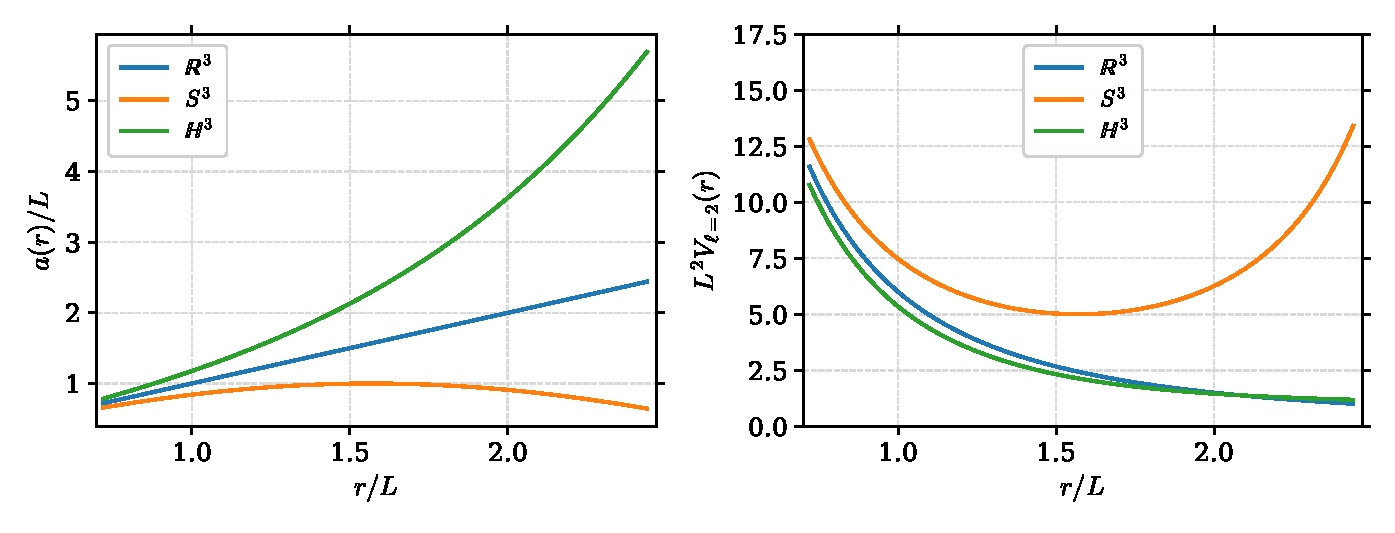
\includegraphics[width=.92\linewidth]{content/MathSkills/figures/geometry-highspin/warped_radial_potentials.pdf}
\caption{同一角动量 $\ell=2$ 在三种三维常曲率空间中的翘曲尺度及酉约化势，均采用 $L=1$。靠近 $r=0$，三者具有相同的 $\ell(\ell+1)/r^2$ 主导奇性；远离原点才可识别不同曲率。图的 $r$ 范围没有延伸到 $S^3$ 的第二极点 $\pi L$。}\label{fig:ghs-r9-warp-potentials}
\end{figure}

\cref{fig:ghs-r9-warp-potentials} 对比了两个不同来源的效应：改变 $a(r)$ 会改变角向面积膨胀；$a''/a$ 则直接给出曲率位移。取 $\ell=0$ 时可再作一个独立的谱核验：在 $S^3$ 上 $u(r)=\sin(r/L)$ 满足两端正则条件并有 $H_0u=0$，对应原始标量 拉普拉斯算子 的常数零模；在 $\mathbb H^3_L$ 上 $V_{0,-}=L^{-2}$，无穷远端是连续谱的阈值，而不是一个可归一化的常数本征态。

对 $S^3$，选定 $\ell\ge0$，引入 $x=r/L$ 与 $n\ge\ell$ 的整数。正则径向解可以写成
\[
 u_{n\ell}(r)=\sin^{\ell+1}x\,C_{n-\ell}^{(\ell+1)}(\cos x),
\]
其中 $C_k^{(\alpha)}$ 是 Gegenbauer 多项式。将 $u=\sin^{\ell+1}x F(\cos x)$ 代入一维方程，利用 $z=\cos x$、$\dd z/\dd x=-\sin x$ 并整理同次幂，可得
\[
 (1-z^2)F''-(2\ell+3)zF'+(n-\ell)(n+\ell+2)F=0.
\]
这是参数 $\alpha=\ell+1$、次数 $n-\ell$ 的 Gegenbauer 方程。

它的多项式解在 $x=0,\pi$ 都正则，且
\[
 H_\ell u_{n\ell}=\frac{n(n+2)}{L^2}u_{n\ell}.
\]
对同一个 $n$，$\ell=0,1,\ldots,n$，每个 $\ell$ 有 $2\ell+1$ 个磁量子数，因而总简并度
\[
 \sum_{\ell=0}^{n}(2\ell+1)=(n+1)^2.
\]
此简并度既由径向边界条件与球谐分解得到，也同 $S^3$ 上标量 拉普拉斯算子 的 $SO(4)$ 表示论结果一致。

它不意味着一般紧致三维流形具有相同简并。

圆锥提供了把几何与径向量子化联系起来的最直接例子，但它也提醒我们：即使截面的谱已经全部算出，径向算子在锥尖处仍可能没有唯一的量子实现。这个问题不能靠“解在原点有限”一句话处理，因为在奇异几何上，平方可积、正则、有限能量及自伴边界条件并不是同一个要求。

令 $g=\dd r^2+r^2h$，$\Sigma$ 维数为 $d-1$，取 $-\Delta_hu_j=\lambda_ju_j$、$\lambda_j\geq0$，并考虑最小耦合 拉普拉斯算子 $-\Delta_g$。
在模态 $\phi=f_j(r)u_j(y)$ 上，由 \cref{eq:ghs-cone-laplace} 得
\begin{equation}\label{eq:ghs-cone-radial-sturm-liouville}
 -f_j''-\frac{d-1}{r}f_j'+\frac{\lambda_j}{r^2}f_j=E f_j.
\end{equation}
径向测度是 $r^{d-1}\dd r$。令 $f_j=r^{-(d-1)/2}v_j$，此替换把该测度准确地变成 $\dd r$，故是 Hilbert 空间的酉变换，而不只是消除一阶导数的技巧。

\begin{proposition}[逆平方径向算子]
在上述酉变换下，\cref{eq:ghs-cone-radial-sturm-liouville} 等价于
\begin{equation}\label{eq:ghs-inverse-square-radial}
 H_{\nu_j}v_j=Ev_j,
 \quad H_\nu=-\frac{\dd^2}{\dd r^2}+\frac{\nu^2-1/4}{r^2},
 \quad \nu_j^2=\lambda_j+\frac{(d-2)^2}{4}.
\end{equation}
\end{proposition}
\begin{proof}
令 $a=(d-1)/2$，则
\[
 f'=r^{-a}(v'-av/r),\quad
 f''=r^{-a}(v''-2av'/r+a(a+1)v/r^2).
\]
代入径向算子后，$v'$ 系数为 $2a-(d-1)=0$。$r^{-2}v$ 的系数为
\[
 -a(a+1)+(d-1)a+\lambda_j
 =\lambda_j+a(a-1)
 =\lambda_j+\frac{(d-1)(d-3)}4.
\]
另一方面，$\nu_j^2-1/4=\lambda_j+[(d-2)^2-1]/4$，两式相同。径向内积也满足
$\int_0^\infty|f|^2r^{d-1}\dd r=\int_0^\infty|v|^2\dd r$，证明该变换保留谱问题所需的 Hilbert 结构。
\end{proof}

靠近 $r=0$，忽略有限 $E$，方程 $H_\nu v=0$ 的 Frobenius 指数满足
$-\alpha(\alpha-1)+\nu^2-1/4=0$，从而 $\alpha=1/2\pm\nu$。对于 $\nu>0$，两支为
\begin{equation}\label{eq:ghs-inverse-square-indicial}
 v_+(r)\sim r^{1/2+\nu},\qquad v_-(r)\sim r^{1/2-\nu}.
\end{equation}
平方可积性直接由 $\int_0^\epsilon r^{2\alpha}\dd r<\infty$ 当且仅当 $\alpha>-1/2$ 决定。所以 $v_+$ 总可积，$v_-$ 仅在 $\nu<1$ 时可积。

\begin{theorem}[非负逆平方系数的锥尖分类]
\label{thm:ghs-inverse-square-endpoint}
对 $\nu\geq0$ 的 $H_\nu$，初始定义域 $C_c^\infty(0,\infty)$，无穷远端为极限点。锥尖 $r=0$ 在 $\nu\geq1$ 时为极限点，因而不需额外的端点自伴参数；在 $0\leq\nu<1$ 时为极限圆，须选取一个自伴边界条件。$\nu=0$ 的第二独立解变为 $r^{1/2}\log r$。
\end{theorem}
\begin{proof}
上面的平方可积计算证明锥尖可积解的个数：$\nu\geq1$ 时只有一支，$0\leq\nu<1$ 时两支均可积。Weyl 极限点/极限圆理论将这一局部计数与相应二阶 Sturm--Liouville 算子的自伴边界条件个数联系起来。无穷远端在本题实逆平方势下是极限点；可以用非实谱参数时的衰减/增长解并由其 Wronskian 不变性检验。对 $\nu=0$，两指数重合，通过 Frobenius 理论取第二支 $r^{1/2}\log r$，两支仍平方可积。故得所述分类。
\end{proof}

假设 $0<\nu<1$，令
\[
 v(r)=A_vr^{1/2+\nu}+B_vr^{1/2-\nu}+o(r^{1/2+\nu}),
\]
对伴随定义域的函数应将其理解为适当的渐近边界迹。在 $[\epsilon,R]$ 上积分分部，得到
\[
 \langle H_\nu v, u\rangle-\langle v, H_\nu u\rangle
 =\bigl[\overline{u'}v-\overline u v'\bigr]_{\epsilon}^{R}.
\]
令 $R\to\infty$、$\epsilon\to0$，内端配对由系数表示为（依照所取法向符号可能整体取负）
\begin{equation}\label{eq:ghs-inverse-square-boundary-form}
 \mathcal B_0(u,v)=2\nu\bigl(\overline{B_u}A_v-\overline{A_u}B_v\bigr).
\end{equation}
使此反厄密边界型消失的极大一维子空间由一个实参数给出，例如 $B=\kappa A$，$\kappa\in\RR\cup\{\infty\}$。量纲为 $[\kappa]=\mathrm{length}^{2\nu}$。不同 $\kappa$ 给出不同的自伴实现；有些扩张可能支持局域束缚态，并引入几何本身没有的长度尺度。

\begin{figure}[htbp]
 \centering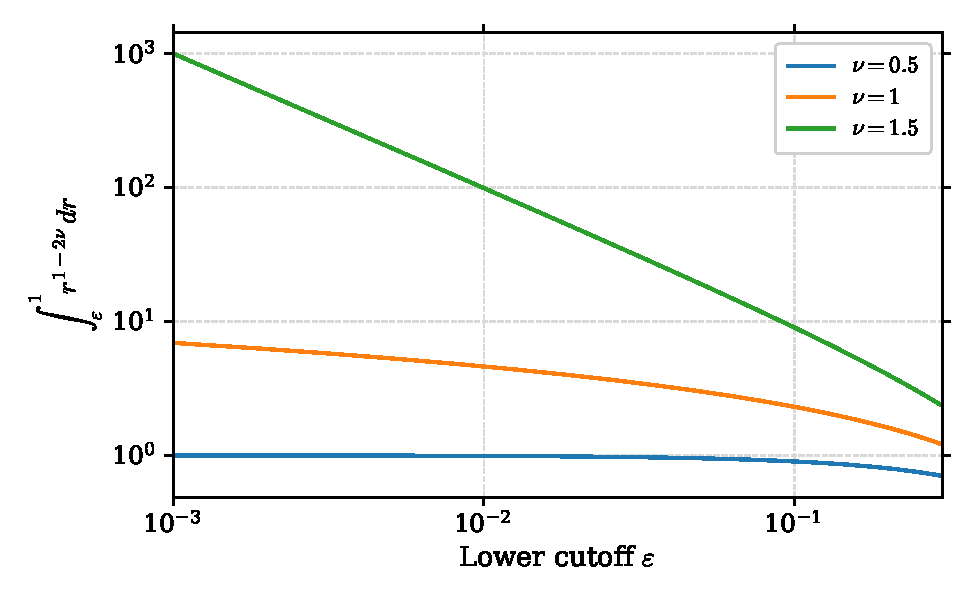
\includegraphics[width=0.77\linewidth]{content/MathSkills/figures/geometry-highspin/conic_boundary_modes.pdf}
 \caption{逆平方径向算子奇异解的截断平方范数。$\nu<1$ 时积分在 $\varepsilon\to0$ 仍有有限极限，$\nu=1$ 呈对数发散，$\nu>1$ 按幂律发散；曲线由 \cref{eq:ghs-inverse-square-indicial} 的幂次精确积分得到。}
 \label{fig:ghs-conic-boundary-norm}
\end{figure}

在平直 $\RR^d$ 去掉原点的 $s$ 波上，$\lambda_0=0$，所以 $\nu_0=(d-2)/2$。当 $d=3$ 时 $\nu_0=1/2<1$，允许非平凡的点相互作用自伴扩张；当 $d=4$ 时 $\nu_0=1$，极限点分类不再给同类单参数族。二维 $d=2$ 时 $\nu_0=0$，必须使用对数支而不是把 $r^{\pm\nu}$ 当作线性独立解。这些结论属于相应径向算子及 Hilbert 空间定义域，而不能被误用为任意相互作用场论的点算符分类。

若圆锥场带曲率耦合 $\xi\mathcal R_g$，则逆平方系数由 $\mathcal R_h$ 改变，且当 $\mathcal R_h$ 不是常数时模态可能发生混合。不能在没有检验这些额外项的情况下直接套用上面的 $\nu_j$。正是这种对定义域与几何条件的明确区分，使任意空间推广具有可检验的数学意义。

抽象谱公式必须通过具体空间检验。不同空间的拓扑、曲率与等距群改变角模态的形式；同一个场算子可以在一种空间上有均匀的角动量阶梯，在另一种空间上只有晶格动量，或者根本不存在方便的显式本征函数。本章固定同一个计算程序，逐次代入不同几何。

取 $\Sigma=S^{d-1}$、单位半径标准度规。曲率 $\mathcal R_h=(d-1)(d-2)$，球谐本征值为 $\lambda_\ell=\ell(\ell+d-2)$。因此
\begin{align}
 A_hY_{\ell a}&=\left[\ell(\ell+d-2)+\frac{(d-2)^2}{4}\right]Y_{\ell a}\nonumber\\
 &=\left(\ell+\frac{d-2}{2}\right)^2Y_{\ell a}.
 \label{eq:ghs-sphere-perfect-square-general}
\end{align}
频率正好是 $\omega_\ell=\ell+\delta$，而不只是它的大 $\ell$ 渐近近似。平方根塌缩成一次函数依赖于圆球曲率与调和谱之间特殊的恒等式。

令球面面积为 $\Omega_{d-1}$、球谐正交归一。对无质量共形标量，柱面两点函数为
\begin{equation}\label{eq:ghs-sphere-cylinder-correlator}
 C(u,\vb n;u',\vb n')
 =\sum_{\ell=0}^\infty\sum_{a=1}^{g_{d,\ell}}
 \frac{\ee^{-(\ell+\delta)|u-u'|}}{2(\ell+\delta)}
 Y_{\ell a}(\vb n)\overline{Y_{\ell a}(\vb n')}.
\end{equation}
将其乘以两端 Weyl 权重 $r^{-\delta}r'^{-\delta}$，回到平直空间时恢复 $|x-x'|^{-(d-2)}$ 类型的二点函数。这个一致性依赖 $d>2$；二维无质量标量具有红外零模和对数关联，不能把 $\delta=0$ 生硬代入振子式。

对严格正的截面算子 $A$，令 $\omega=\sqrt A$。全实直线上的柱体算子 $-\partial_u^2+A$ 有逆核
\begin{equation}\label{eq:math-ghs-positive-cylinder-kernel}
 C_A(u,u')=\frac{\exp[-|u-u'|\sqrt A]}{2\sqrt A}.
\end{equation}
这是谱定理给出的逐模逆算子：对 $Au_j=\lambda_ju_j$，核为
\[
 C_A(u,y;u',y')=\sum_j\frac{\ee^{-\sqrt{\lambda_j}|u-u'|}}{2\sqrt{\lambda_j}}
 u_j(y)\overline{u_j(y')}.
\]
每一项在 $u\ne u'$ 时解齐次方程，一阶导数在 $u=u'$ 的跃变为 $-1$，故产生单位 $\delta(u-u')$ 源。零模必须单独处理，负谱不能给出这种衰减正核。该逆核作为自由量子场协方差的解释见《自由电子量子光学》的几何自由场章节。

取 $(d-1)$ 维平直环面 $T^{d-1}=\RR^{d-1}/(L_1\ZZ\oplus\cdots\oplus L_{d-1}\ZZ)$，体积 $V=\prod_aL_a$，用周期坐标 $y^a$。归一化本征函数和谱为
\begin{equation}\label{eq:ghs-torus-spectrum}
 u_{\vb k}(y)=V^{-1/2}\ee^{\ii\sum_a2\pi k_ay^a/L_a},\quad
 -\Delta_hu_{\vb k}=\left(\sum_a\frac{4\pi^2k_a^2}{L_a^2}\right)u_{\vb k},\quad \vb k\in\ZZ^{d-1}.
\end{equation}
若加入正质量 $m_0>0$，频率是 $\omega_{\vb k}=\sqrt{m_0^2+\sum_a(2\pi k_a/L_a)^2}$。协方差由 \eqnrefs{eq:math-ghs-positive-cylinder-kernel} 立刻得到
\[
 C_T(u,y;u',y')=\frac1V\sum_{\vb k\in\ZZ^{d-1}}
 \frac{\ee^{-\omega_{\vb k}|u-u'|+\ii\sum_a2\pi k_a(y^a-y'^a)/L_a}}{2\omega_{\vb k}}.
\]
现在模态由整数晶格向量标记。其简并来自格点的长度相等，而非 $SO(d)$ 高自旋表示。若 $L_a$ 一般互不相等，除 $\vb k\leftrightarrow-\vb k$ 外通常没有球面式的大简并。

设 $\Sigma$ 为维数 $d-1$ 的紧致负 Einstein 截面，$\mathcal R_h<0$。常数模 $u_0=V^{-1/2}$ 给出
\[
 A_hu_0=\xi_d\mathcal R_hu_0.
\]
当 $d>2$，本征值为负。尽管圆锥上的无质量方程仍能通过 Weyl 协变性转换成柱面方程，该负模不能被解释为有稳定真空的正频振子。若将局部质量项 $m_0^2$ 加到柱面算子，则需要 $m_0^2> -\inf\operatorname{spec}(A_h)$ 才能使用 \eqnrefs{eq:math-ghs-positive-cylinder-kernel}；这改变了原先共形无质量模型，不能称其为同一个共形场论。

\begin{figure}[htbp]
 \centering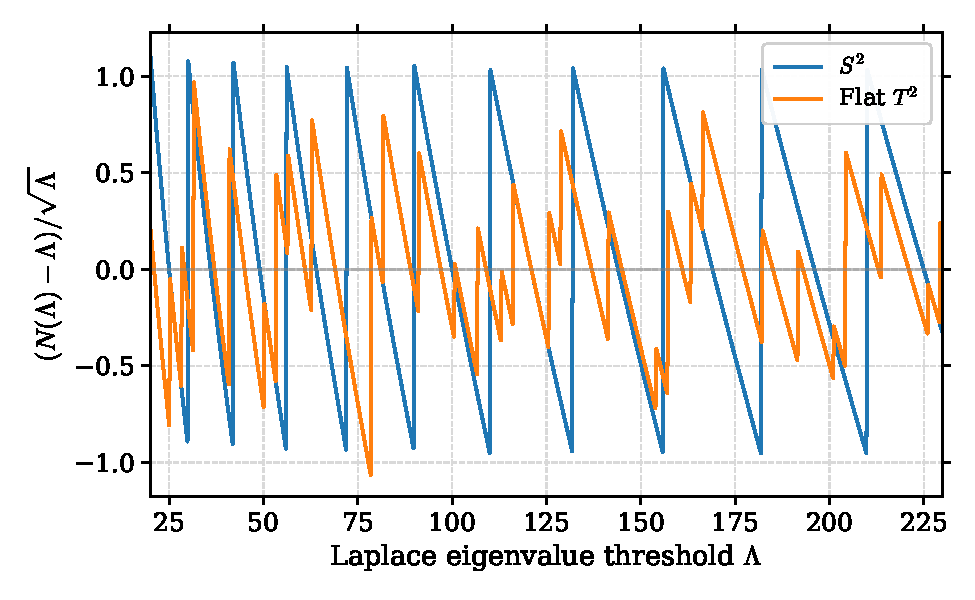
\includegraphics[width=0.78\linewidth]{content/MathSkills/figures/geometry-highspin/sphere_torus_spectral_residual.pdf}
 \caption{面积同为 $4\pi$ 的单位二球面与正方形平直环面之谱计数阶梯，减去相同的 Weyl 主项 $N(\Lambda)\sim\Lambda$ 后除以 $\sqrt\Lambda$。球面的大简并产生较规则的阶梯，环面的格点计数呈另一种振荡；两者有相同领先态密度，却没有相同的精确谱。}
 \label{fig:ghs-sphere-torus-residual}
\end{figure}

取正弦翘曲积
$g=\dd r^2+R^2\sin^2(r/R)\,\dd\Omega_{d-1}^2$，$0<r<\pi R$。它是圆球去掉两极后的度规；两个端点的球面会塌缩，不能用同一组固定截面来构造整个紧致球上的全局圆柱时间。局部变量 $u=\log\tan(r/(2R))$ 给出
\[
 \sin(r/R)=\frac1{\cosh u},\qquad
 g=\frac{R^2}{\cosh^2u}(\dd u^2+\dd\Omega_{d-1}^2).
\]
该几何与柱面共形相关，而不是等距相同。对于质量为零且采用共形耦合的经典标量，Weyl 协变性使柱面算子仍可对角化；量子关联函数还需指定在紧致球两端的正则条件与 Weyl 异常处方。

将这一特殊翘曲函数代回度规，便得到相应的柱面坐标。
由 $u=\log\tan(r/(2R))$ 求导，
\[
 \frac{\dd u}{\dd r}=\frac1{R\sin(r/R)},\qquad
 \dd r=R\sin(r/R)\dd u.
\]
因此 $\dd r^2+R^2\sin^2(r/R)\dd\Omega^2=R^2\sin^2(r/R)(\dd u^2+\dd\Omega^2)$。再使用
$\tan(r/(2R))=\ee^u$ 与 $\sin(2\arctan z)=2z/(1+z^2)$，得到
$\sin(r/R)=2\ee^u/(1+\ee^{2u})=1/\cosh u$。将系数代回即得所列度规。由此可见球面两极在柱面上分别位于 $u\to\mp\infty$。

对于任何给定的紧致截面，先选定 $h$、场所处向量丛、相关二次型及算子定义域；随后求自伴实现 $A$ 的谱或谱测度，并检查其下界。若存在等距群，则优先把 Hilbert 空间按不可约表示分块以简化 $A$；若不齐性则用有限元、谱方法或热核渐近求解。最后根据 \eqnrefs{eq:math-ghs-positive-cylinder-kernel} 构造自由关联函数。只有当几何还提供守恒的尺度生成元和合适的局域算符扇区时，才把该谱进一步解释为共形维数。

\subsection{分离变量的前提}

若 $g=\dd r^2+a(r)^2h$ 且 $A_hu_j=\lambda_ju_j$，对 $\phi(r,y)=f_j(r)u_j(y)$ 代入
$(-\Delta_g+m^2+\xi\mathcal R_g)\phi=0$，得到
\[
 -f_j''-(d-1)\frac{a'}a f_j'
 +\left(\frac{\lambda_j-\xi\mathcal R_h}{a^2}
 +m^2+\xi\mathcal R_g\right)f_j=0,
\]
其中使用 $-\Delta_hu_j=(\lambda_j-\xi\mathcal R_h)u_j$ 要求 $\mathcal R_h$ 为常数；若其不是常数，必须改用 $-\Delta_h$ 的本征基来做 Laplace 分离，或者在相应基底内保留曲率势矩阵。即使可以分离变量，端点附近的正规条件也关系到径向微分算子的自伴实现。

\subsection{算符与量纲}

若物理截面为 $R^2h$，本征值缩放为 $\lambda_j^{\rm phys}=R^{-2}\lambda_j$，真实频率为 $\Omega_j=c\sqrt{\lambda_j}/R$（无量纲 $\lambda_j$ 包含正质量/曲率项）。量子能量激发为 $\hbar\Omega_j$。这与圆柱谱的单位恢复完全一致；但在随时间变化的空间中，不可用单个 $\Omega_j$ 标记全程的能量本征态。

\section{柱体边界响应与拼接}

现在令 $\Sigma$ 为紧致无边界截面，$B\ge0$ 为其上自伴椭圆算子，在有限柱体 $[0,L]\times\Sigma$ 上考虑
\begin{equation}\label{eq:ghs-r6-cylinder-elliptic}
(-\partial_t^2+B)u=0,\qquad u(0)=f_0,\quad u(L)=f_L.
\end{equation}
边界值虽然只落在两张超曲面上，却已经决定了内部的经典场。这说明边界作用量能够编码内部传播；相应的线性算子是 Dirichlet--to--Neumann 映射。


\begin{theorem}[有限柱体的精确边界算子]\label{thm:ghs-r6-cylinder-dn}
在 $B$ 的严格正谱上，外法向边界数据 $(-\partial_tu(0),\partial_tu(L))$ 等于
\begin{equation}\label{eq:ghs-r6-dn-matrix}
\begin{pmatrix}\sqrt B\coth(L\sqrt B)&-\sqrt B\operatorname{csch}(L\sqrt B)\\
-\sqrt B\operatorname{csch}(L\sqrt B)&\sqrt B\coth(L\sqrt B)\end{pmatrix}
\begin{pmatrix}f_0\\f_L\end{pmatrix}.
\end{equation}
零本征子空间上的同一矩阵按连续极限解释为 $L^{-1}\begin{psmallmatrix}1&-1\\-1&1\end{psmallmatrix}$。该映射对称且非负。
\end{theorem}
\begin{proof}
取 $Bu_j=\lambda_ju_j$，写 $u(t,y)=\sum_jq_j(t)u_j(y)$。对 $\lambda_j>0$ 令 $\omega_j=\sqrt{\lambda_j}$，边值常微分方程 $-q_j''+\omega_j^2q_j=0$ 的唯一解为
\[
q_j(t)=\frac{\sinh[\omega_j(L-t)]}{\sinh(\omega_jL)}f_{0j}
+\frac{\sinh(\omega_jt)}{\sinh(\omega_jL)}f_{Lj}.
\]
分别对 $t$ 求导并取端点，得到
\[
-q'_j(0)=\omega_j\coth(\omega_jL)f_{0j}
-\omega_j\operatorname{csch}(\omega_jL)f_{Lj},
\]
\[
q'_j(L)=-\omega_j\operatorname{csch}(\omega_jL)f_{0j}
+\omega_j\coth(\omega_jL)f_{Lj}.
\]
再由谱演算重组为矩阵式。$\omega_j\to0$ 时 $q_j$ 变成端点的线性插值，故零模矩阵具有所给极限。将方程乘以 $\bar u$ 积分分部得到
\[
\langle \Lambda_L(f_0,f_L),(f_0,f_L)\rangle
=\int_0^L\!\bigl(\norm{\partial_tu(t)}^2+\langle Bu(t), u(t)\rangle\bigr)\dd t\ge0,
\]
从而非负性与对称性均可直接验证。严格连续边界算子应理解为适当的 Sobolev 迹空间之间的映射；上述模态计算先在有限谱截断上成立，再由闭二次型扩张。
\end{proof}

离散化后的高斯路径积分把内部变量消去，正是对二次型取 Schur 补；而这里的连续精确边界算子给出了这个代数步骤的几何含义。不同的边界条件会改变谱和高斯归一化，故“内部积分掉了，所以只剩同一个有效作用量”的说法一般不成立。

几何算子提供了谱、逆核和边界二次型；当场论还具有时空对称性，下一章的 Noether 理论才将这些微分结构联系到守恒荷。
